\subsection{Sensory Motor Network is a Sensation Modulating Network}

In the previous sections we drew a sketch of the architecture of the cognitive agent in terms of polarized, tubular, segmented, bilaterally symmetrical, antagonistic organization. On to that architectural scaffolding, the cognitive organs are `mounted'. Consider this as another layer of describing the same body, but underlining the cognitive features of the agent.

The three components of concern for a cognitive architecture are (1) the sensory receptors organised as \textit{sensory boards (SB)}, (2) the motor action zones organised as \textit{motor boards (MB)} and (3) the connectors in between sensory and motor boards organised as a \textit{network}. Thus the body of a cognitive agent is modelled as a sensation modulating network (SMN). The nodes of the network include sensory and motor boards, while the edges include the connections of the network. Biologically, sensory boards are realised by sensory receptors, motor boards by the muscular and skeletal system and the edges of the network (connections) by the nervous system.

It is important to keep in mind the contrasting point of the architecture with the received view that confines network only to the nervous systems, where the body of the neuron, the soma, forms the node, and the axons and dendrites form the connections. In our model, the entire cognitive agent's body is a network, with the nervous system providing only the differential connections between different sensory-motor subsystems. 

Sensory receptors are located in a distributed way across the body in the outer, inner and middle layers. The distribution of these nodes \textit{on} and \textit{in} the body is not uniform. Polarization exists, in the sense that some nodes are arranged densely on one-side of the tube. For example, a pair of eyes are located towards one pole of the body and absent at other places. Each eye has multiple photo-receptors and motor modulators, together constituting the nodes of the network. Similarly we see such concentrations of sensory receptors for other modalities. Although tactile receptors are located in a distributed way, their density varies from place to place on and in the body. This unequal distribution in location and density of sensory receptors plays an important role in differentiation and solving the problem of location.

The sensory receptors are differentiated into specialised modalities transducing thermal, tactile, auditory, visual, olfactory, gustatory and location signals. The polarised and bilaterally symmetrical arrangement of these sensory receptors plays a significant role in constructing the picture of the internal and external world. The receptors organised as sensory boards are \textit{mounted} on the motor and mechanical boards (muscular and skeletal system). One more contrasting point of this model may be noted, that we consider the motor boards as sensory receptors of location, and not merely as actuators. As far as cognition is concerned, actuation is essentially for supporting sensation of every modality, committing to the theory of action based perception. 

On this body plan, there are also multiple action zones. It is important to note that action zones are also oriented towards the inner layers of the tubular body plan of the agent. There are more action zones at the anterior side, particularly at the inner surface of the tube, making the body polarized. Animal anatomy describes this plan often in the name of cephalization \cite{hyman1940invertebrates}, seen in almost all bilaterally symmetric beings. 

Apart from the polarised distribution of sensory organs, it is important to note that the motor organs, which are also sense organs, are located in a \textit{nested} manner across the body.

A large set of highly specialized motor receptors (location sensors), are present across the body organized in a bilaterally symmetrical and hierarchical (nested) manner, which biologists call as skeletal or voluntary muscles. In our model, insofar as cognition is concerned, skeletal muscles are sense organs, and their movement directly supports perception. Biologically, muscles are considered as organs of movement and locomotion. In conventional cognitive science, their role is considered auxiliary. In our model, movement and locomotion are primarily cognitive functions. Apart from providing location data as a sensory subsystem, their \textit{characteristic} movement provides conceptual schemes employed in cognition.

The motor receptors of the network are unique, because they are mounted/embedded in a bundle of muscle fibres organised as \textit{boards}. This specialized plan is essential for playing the role of \textit{inferring} the location. The data from location sensors is created through movement. That is to say, the position is resolved only by change-in-position (displacement). But, location cannot be determined without data from the other sensory streams. We interpret location, like consciousness, as a dispositional concept. Location is always of some thing or the other, some sensation or the other, of some phenomena or the other. Employing a Kantian aphorism, we may say: location without sensory data is empty, and sensory data without location is blind. Moreover, it is not only that location cannot be calculated without movement, the construction of an image of the world through other senses is impossible without spatio-temporal data. Action is essential for resolving both space and time.  

The source of temporal data is the serial action pattern.The body plan is not only polarised and nested, but also serial in nature. We also assume availability of repeatable actions, beats within the body, providing a temporal canvas/ stage. The availability of the temporal stage/ canvas is granted by the existence of metabolic cycles, biological clocks is well established [cite] in terms of diurnal and biurnal rhythms.

Antagonistic action is a key character of the body plan, which plays an important role in the current model. 

The body is not a complete network. The model uses the principle: ``Fire together. Wire together'' (FTWT) \cite{hebb1949organisation}. The SMNs that are recurrently active at the same time are likely to get connected over a period of time. Thus the connection `board' is plastic, not static. The connection patterns are created, reinforced and modified based on the dynamics of the body (action patterns) in its ontogeny (developmental history). The implication of the FTWT principle is that the actions determine the connections, and not the other way around. However, much of the differential connections may have been already determined by phylogenetic and prenatal action history. Though it appears as though the agent starts with an undifferentiated state, the phylogenetic and prenatal action history bestows, practically, a body with `innate' action schemas at birth.

In a model where actions are located at the interface between the body and the environment, the actions within the body (including the prenatal stage) are often ignored (e.g. suckling, swallowing action-patterns etc.). In our model, the most stable and determining action schemas are already in place by the time the agent is exposed to the external environment after birth. 

\begin{figure}[ht] 
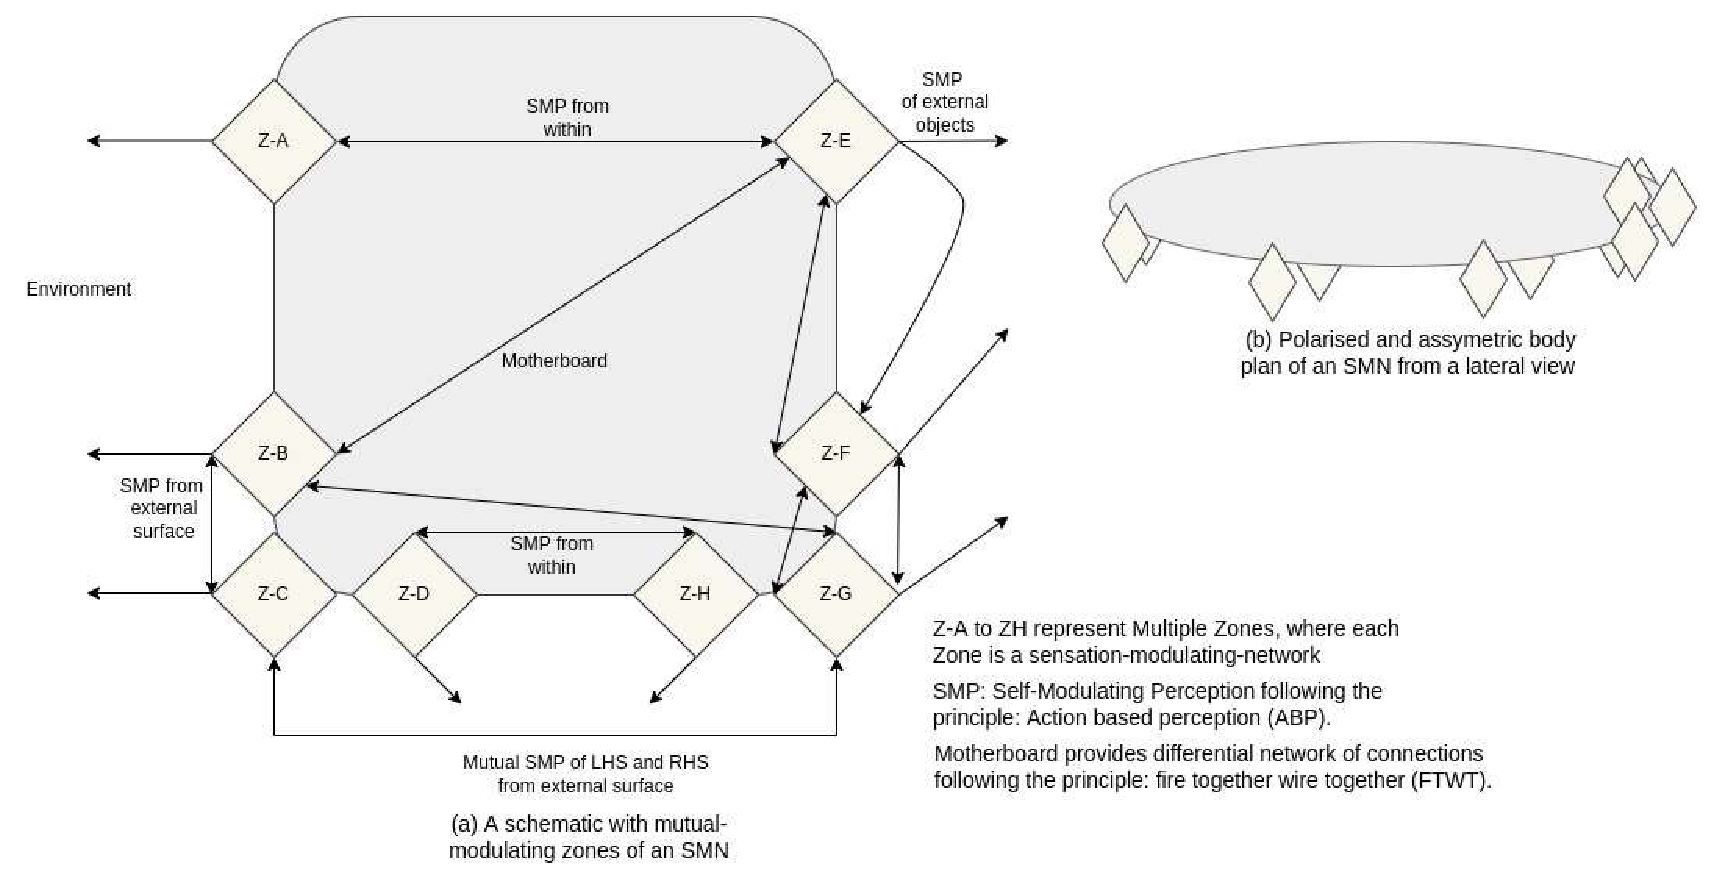
\includegraphics[width=\textwidth]{graphics/self-modulating-perception.pdf}
\caption{\textbf{A schematic representing a cognitive agent as a network of multiple self-modulatable zones.}}
\label{smn}
\end{figure}

Mutual modulation of action within the body is an important and contrasting feature of the model, which is largely ignored in the current discussions in cognitive science. This mutual modulation, within the body, is a core cognitive mechanism in the current model, which appears very early on during the prenatal stage itself. Therefore, we locate the roots of cognition within mutual modulation within the body (internal environment).

The outgoing arrows from the zones represent the sensory modulation from an external world invoking action based perception (ABP) \cite{noe_action_2004}. According to this principle, the perception is not a passive sensing of the world out there, but an active process. The same principle is employed when an action zone modulates another action zone within the body. This implies that ABP is used for perceiving both the worlds (internal and external). The double headed arrows in the figure represent mutually modulating zones. Between Z-B and Z-C, the double-headed arrow represents mutual modulation from the outer surface. For example, consider a fidgeting action between fingers touching side-ways, the hand touching the chin in the typical thinking posture, scratching an itch on the same side of the body etc. The double-headed arrow between Z-C and Z-G represents another mutual modulation from an outer surface (e.g. clapping with hands), LHS and RHS mutually modulating.

In a well-connected body, the implementation of a single-headed arrow between two zones (like Z-E and Z-F) appears very rare. However, to understand such a possibility, we can consider touching a numb leg, where due to temporary lack of internal feedback, mutual modulation is transiently unavailable. The double-headed arrow between Z-D and Z-H could represent mutual modulation between the action zones from within the body. For example, swallowing zone and speech zone. In the case of swallowing, with or without food, the upper and lower surfaces of the buccal cavity, pharyngeal zones mutually touch and modulate each other.

Often, self modulating actions, such as thinking, are considered as recent evolutionary features, whereas in our model, the very root of cognition is due to such internal mutual modulation, though it is counter-intuitive. The world within the body is missed in the current accounts. Since this is a contrasting feature, more elaboration on this follows in the model. 

\begin{figure}[ht] 
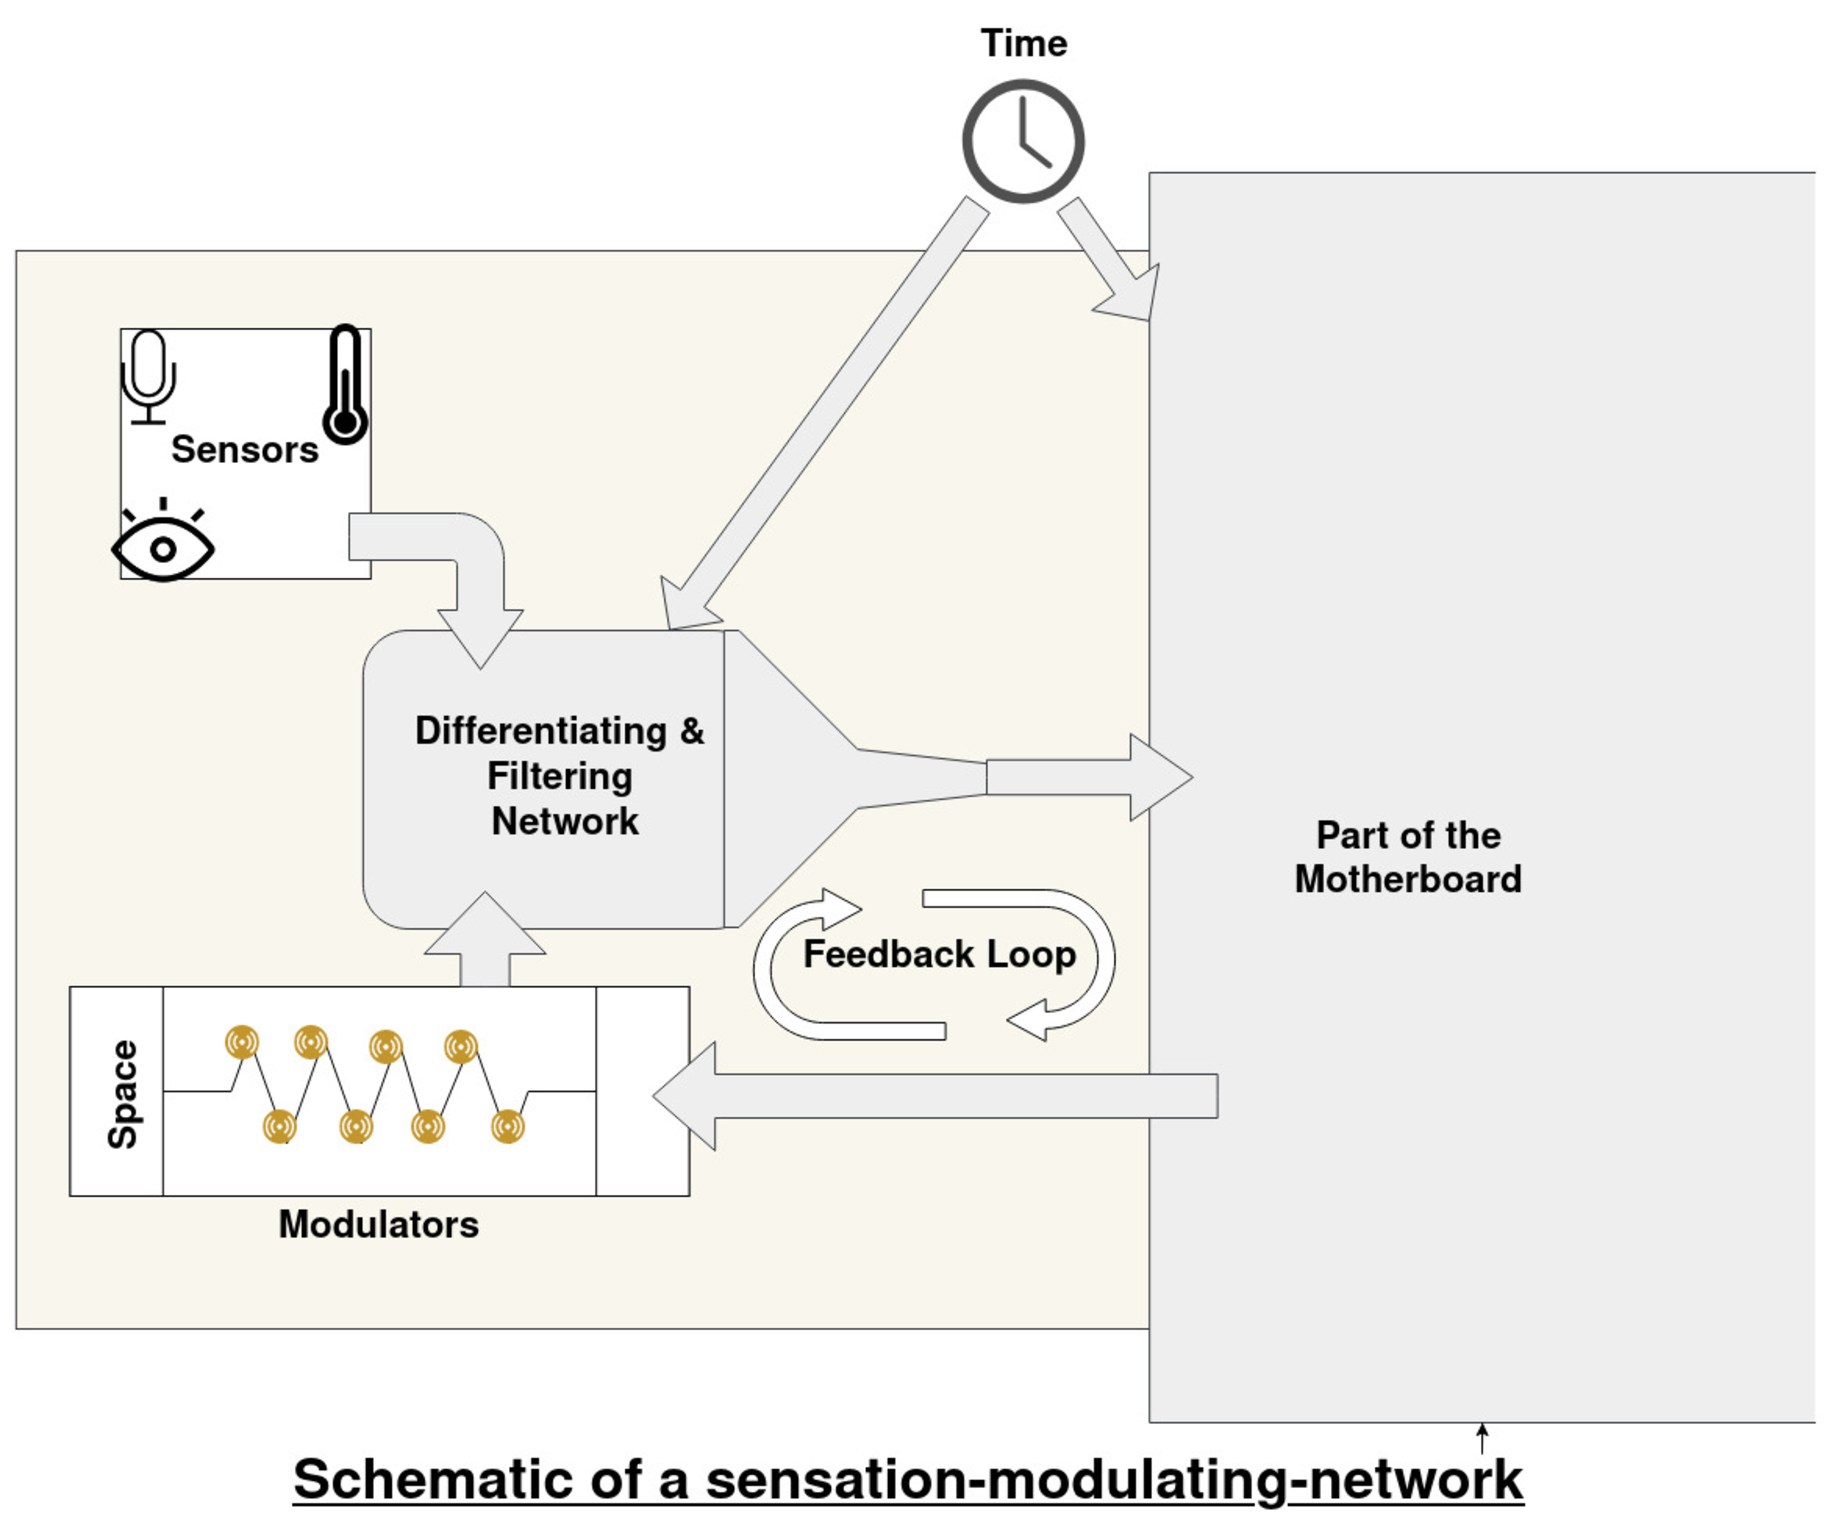
\includegraphics[width=\textwidth]{graphics/structure-of-Zone.pdf}
\caption{\textbf{A schematic of a perception modulating action zone.}}
\label{zone}
\end{figure}

\subsection{A Network of Sensation modulating networks}

The structure of a cognitive agent's body is modeled as a nested network of Sensation Modulating Networks $\{n(SMN)\}$. And the dynamics of cognition is modeled as differentiation of Differences $\{\delta(D)\}$ in a  multi-modal sensory stream.

It is important to underline, as a point of contrast, that the Central Nervous System (CNS) is not interpreted as \textit{the} network in our model, but a part of it. The entire cognitive agent's body is a network. CNS provides only the differential connections between different DFNs and among the nodes (sensory and motor receptors). Therefore the popular schema of brain-body-world is reduced to body-world. Since the body is a network of SMN, this schema can be represented as 
\begin{equation}
[\{n(SMN)\} \rightleftharpoons \{W_I\}] \rightleftharpoons \{W_E\},
\end{equation}

where $W_I$ is the internal world and $W_E$ is the external world.  $W_I$ can be substituted with another $\{n(SMN)\}$, since it is nothing but another $W_I$ in effect. 

Thus the above representation can be re-written as 
\begin{equation}
[\{n(SMN)\}_i \rightleftharpoons \{n(SMN)\}_j] \rightleftharpoons \{W_E\}.
\end{equation}
What constitutes the internal world will become clear once we make the principle of mutual modulation clear below.

This schema can be contrasted with the brain-body-world schema, which can be represented as 

\begin{equation}
\{CNS\} \rightleftharpoons \{B\} \rightleftharpoons \{W_E\}
\end{equation}

where the CNS is the central nervous system, B is the rest of body and $W_E$ is the external world.

Consider the functional network as a $\Delta$ network of a set of sensory boards $\{S_i\}$ and motor boards $\{M_j\}$. We represent this network as 
\begin{equation}\label{delta_notation}\Delta^{\{S_i\}}_{\{M_j\}}, or simply, as  \Delta^{\{i\}}_{\{j\}},
\end{equation} 
where the subscripts always refer to motor boards, and superscripts to the sensory boards. For example, if $S_1$, $S_2$, $S_4$ and $M_1$, $M_5$, constitute a transient network at any given time $t_1$, this state of the SMN can be represented as 
\begin{equation}\label{delta_eg}SMN(t_1) = \Delta^{1,2,4}_{1,5}
\end{equation} 
This $\Delta$ network is an ephemeral functional state corresponding to a particular action performed by the cognitive agent at $t_1$. Thus differentiation of Differences is realised in $\Delta$ networks, where the motor boards differentiate on the Differences streaming from the multi-modal sensory boards. This is how we resolve every action as a functional network of sensory motor subsystems.

Differences are given and taken from the environment directly, while differentiation is an active function of the agent. This active function can resolve modalities and selectively attend to a difference in the stream.

SMNs are functional states of the cognitive agent. This identifiable functional state does differentiation and filtering. Since each SMN is a network, the body is a network of networks. We may represent the active cognitive agent as $\{n(SMN)\}$. The first order network of SMN is a functional sub-graph. By functional subgraph, we mean, it is not distinguished based on structure, but by ephemeral or transient connections. SMN is hence localizable, but ephemerally.

Each sensory board is an array of localised sensory receptors (transducers), which connect through a bundle of connectors (a bus) to a differentiating and filtering network (DFN). Each motor board is an array of location-receptors mounted on a bundle of actuators (muscle-fibers). The motor board connects through a bundle of connectors to the DFN on the one hand, and receives connections from the integrating network (IN) on the other. The DFN and IN are distinguishable only on the basis of their function and the nature of connections, and need not be localized in any specific area of the central nervous system (CNS).

The motor board can be considered as a mediating board between a DFN and IN. In other words, the motor board is sandwiched between the DFN and IN, creating dynamic and transient loops. Speaking of the network in graph-theoretic terms, we can say that, the nodes of an SMN are arrays of receptors and actuators, and the edges are dynamically distributed bundles of connections manifesting the aforementioned loop.

\begin{equation}
[\{n(SMN)\}_i \rightleftharpoons \{n(SMN)\}_j] \rightleftharpoons \{W_E\}.
\end{equation}
What constitutes the internal world will become clear once we make the principle of mutual modulation clear below.


This schema can be contrasted with the brain-body-world schema, which can be represented as 

\begin{equation}
\{CNS\} \rightleftharpoons \{B\} \rightleftharpoons \{W_E\}
\end{equation}

where the CNS is the central nervous system, B is the rest of body and $W_E$ is the external world.

%=== Empirical hooks ===
\paragraph{Empirical hooks.}
The SMN commitments align with: (i) lawful coordination dynamics and phase-transitions in interlimb control \citep{HakenKelsoBunz1985,Kelso1995}; 
(ii) nested neural oscillations that gate sensorimotor sampling and rephasing \citep{Buzsaki2006}; 
(iii) interrupt/stop paradigms demonstrating rapid, safe halting and task re-routing \citep{Aron2007}; and 
(iv) muscle-synergy composition as a substrate for modular control with low-dimensional reconfiguration \citep{BizziCheung2013}. 
Together these illustrate how interruptibility, composition, and affordance-based guarding instantiate cognitive control without presupposing disembodied symbol manipulations.

